% ====================================================================
% Software Reengineering Project Report
% Point-of-Sale System Reengineering
% ====================================================================

\documentclass[12pt,a4paper]{report}

% ====================================================================
% Packages
% ====================================================================
\usepackage[utf8]{inputenc}
\usepackage[T1]{fontenc}
\usepackage{geometry}
\usepackage{graphicx}
\usepackage{booktabs}
\usepackage{longtable}
\usepackage{array}
\usepackage{multirow}
\usepackage{xcolor}
\usepackage{listings}
\usepackage{hyperref}
\usepackage{fancyhdr}
\usepackage{titlesec}
\usepackage{tocloft}
\usepackage{caption}
\usepackage{subcaption}
\usepackage{float}
\usepackage{enumitem}
\usepackage{amsmath}
\usepackage{amssymb}
\usepackage{tikz}
\usepackage{forest}
\usetikzlibrary{shapes.geometric, arrows, positioning, fit, calc}

% ====================================================================
% Page Setup
% ====================================================================
\geometry{
    left=2.5cm,
    right=2.5cm,
    top=2.5cm,
    bottom=2.5cm
}

% ====================================================================
% Colors
% ====================================================================
\definecolor{codegreen}{rgb}{0,0.6,0}
\definecolor{codegray}{rgb}{0.5,0.5,0.5}
\definecolor{codepurple}{rgb}{0.58,0,0.82}
\definecolor{backcolour}{rgb}{0.95,0.95,0.92}
\definecolor{fastblue}{RGB}{0,51,102}
\definecolor{fastgold}{RGB}{255,204,0}

% ====================================================================
% Code Listing Style
% ====================================================================
\lstdefinestyle{mystyle}{
    backgroundcolor=\color{backcolour},   
    commentstyle=\color{codegreen},
    keywordstyle=\color{blue},
    numberstyle=\tiny\color{codegray},
    stringstyle=\color{codepurple},
    basicstyle=\ttfamily\footnotesize,
    breakatwhitespace=false,         
    breaklines=true,                 
    captionpos=b,                    
    keepspaces=true,                 
    numbers=left,                    
    numbersep=5pt,                  
    showspaces=false,                
    showstringspaces=false,
    showtabs=false,                  
    tabsize=2,
    frame=single
}
\lstset{style=mystyle}

% Python style
\lstdefinelanguage{Python}{
    keywords={def, class, return, if, else, elif, for, while, try, except, with, as, import, from, True, False, None, self, and, or, not, in, is, lambda, yield, raise, finally, pass, break, continue, global, nonlocal, assert, del},
    keywordstyle=\color{blue}\bfseries,
    ndkeywords={int, str, float, bool, list, dict, tuple, set, Optional, List, Dict},
    ndkeywordstyle=\color{codepurple}\bfseries,
    identifierstyle=\color{black},
    sensitive=true,
    comment=[l]{\#},
    morecomment=[s]{'''}{'''},
    morecomment=[s]{"""}{"""},
    commentstyle=\color{codegreen}\ttfamily,
    stringstyle=\color{red}\ttfamily,
    morestring=[b]',
    morestring=[b]"
}

% Java style
\lstdefinelanguage{Java}{
    keywords={abstract, assert, boolean, break, byte, case, catch, char, class, const, continue, default, do, double, else, enum, extends, final, finally, float, for, goto, if, implements, import, instanceof, int, interface, long, native, new, package, private, protected, public, return, short, static, strictfp, super, switch, synchronized, this, throw, throws, transient, try, void, volatile, while, true, false, null},
    keywordstyle=\color{blue}\bfseries,
    sensitive=true,
    comment=[l]{//},
    morecomment=[s]{/*}{*/},
    commentstyle=\color{codegreen}\ttfamily,
    stringstyle=\color{red}\ttfamily,
    morestring=[b]",
}

% ====================================================================
% Header and Footer
% ====================================================================
\pagestyle{fancy}
\fancyhf{}
\fancyhead[L]{\leftmark}
\fancyhead[R]{Software Reengineering}
\fancyfoot[C]{\thepage}
\renewcommand{\headrulewidth}{0.4pt}
\renewcommand{\footrulewidth}{0.4pt}

% ====================================================================
% Hyperref Setup
% ====================================================================
\hypersetup{
    colorlinks=true,
    linkcolor=fastblue,
    filecolor=magenta,      
    urlcolor=cyan,
    citecolor=blue,
    pdftitle={POS System Reengineering Report},
    pdfauthor={Muhammad Ahmad, Usaid Afzal},
}

% ====================================================================
% Title Formatting
% ====================================================================
\titleformat{\chapter}[display]
    {\normalfont\huge\bfseries\color{fastblue}}{\chaptertitlename\ \thechapter}{20pt}{\Huge}
\titleformat{\section}
    {\normalfont\Large\bfseries\color{fastblue}}{\thesection}{1em}{}
\titleformat{\subsection}
    {\normalfont\large\bfseries}{\thesubsection}{1em}{}

% ====================================================================
% Document Begin
% ====================================================================
\begin{document}

% ====================================================================
% Title Page
% ====================================================================
\begin{titlepage}
    \centering
    \vspace*{1cm}
    
    % University Logo (placeholder)
    \includegraphics[width=0.3\textwidth]{example-image}
    
    \vspace{1cm}
    
    {\LARGE\textbf{FAST National University of Computer \& Emerging Sciences}}
    
    \vspace{0.5cm}
    
    {\Large Islamabad Campus}
    
    \vspace{1.5cm}
    
    {\Huge\textbf{\color{fastblue}Software Reengineering}}
    
    \vspace{0.5cm}
    
    {\LARGE\textbf{Project Report}}
    
    \vspace{1cm}
    
    {\Large\textbf{Point-of-Sale System Reengineering}}
    
    \vspace{0.3cm}
    
    {\large Transforming Legacy Desktop Application to Modern Web-Based System}
    
    \vspace{2cm}
    
    \begin{tabular}{ll}
        \textbf{Submitted By:} & \\
        & Muhammad Ahmad (22i-2711) \\
        & Usaid Afzal (22i-8783) \\
        \\
        \textbf{Section:} & SE-G \\
        \textbf{Semester:} & Fall 2025 (7th Semester) \\
    \end{tabular}
    
    \vfill
    
    {\large\textbf{December 2025}}
    
\end{titlepage}

% ====================================================================
% Table of Contents
% ====================================================================
\tableofcontents
\newpage

\listoffigures
\listoftables
\newpage

% ====================================================================
% Chapter 1: Introduction
% ====================================================================
\chapter{Introduction}

\section{Project Overview}

This report presents the complete software reengineering of a legacy desktop-based Point-of-Sale (POS) system. The original system was developed in Java using Swing GUI framework and stored data in plain text (.txt) files. Through systematic application of the Software Reengineering Process Model, we have transformed this legacy application into a modern, web-based system with improved architecture, documentation, data management, and maintainability.

\section{Objectives}

The primary objectives of this project are:
\begin{enumerate}
    \item \textbf{Inventory Analysis} -- Identify, classify, and assess existing software assets
    \item \textbf{Document Restructuring} -- Reorganize and recreate technical documentation
    \item \textbf{Reverse Engineering} -- Recover design, data structures, and logic from existing codebase
    \item \textbf{Code Restructuring} -- Improve maintainability and readability of legacy code
    \item \textbf{Data Restructuring} -- Redesign and migrate data from plain-text to database
    \item \textbf{Forward Engineering} -- Develop improved web-based application
\end{enumerate}

\section{Legacy System Overview}

The original POS system was a Java Swing desktop application with the following characteristics:
\begin{itemize}
    \item \textbf{Language:} Java SE 8+
    \item \textbf{GUI Framework:} Java Swing (javax.swing.*)
    \item \textbf{Data Storage:} Plain text files (.txt)
    \item \textbf{Architecture:} Monolithic, tightly coupled
    \item \textbf{Lines of Code:} Approximately 2,700+ lines
    \item \textbf{Source Files:} 17 Java files
\end{itemize}

\section{Report Structure}

This report is organized following the phases of the Software Reengineering Process Model:
\begin{itemize}
    \item Chapter 2: Inventory Analysis
    \item Chapter 3: Document Restructuring
    \item Chapter 4: Reverse Engineering
    \item Chapter 5: Code Restructuring
    \item Chapter 6: Data Restructuring
    \item Chapter 7: Forward Engineering
    \item Chapter 8: Refactoring Documentation
    \item Chapter 9: Risk Analysis \& Testing
    \item Chapter 10: Technology Justification
    \item Chapter 11: Conclusion
\end{itemize}

% ====================================================================
% Chapter 2: Inventory Analysis
% ====================================================================
\chapter{Inventory Analysis}

\section{Executive Summary}

The Inventory Analysis phase identifies, classifies, and assesses all existing software assets in the legacy POS system. This systematic cataloging provides the foundation for all subsequent reengineering activities.

\section{Software Asset Inventory}

\subsection{Source Code Files}

Table \ref{tab:source-files} presents the complete inventory of Java source files in the legacy system.

\begin{longtable}{|l|c|l|p{5cm}|}
\caption{Source Code File Inventory} \label{tab:source-files} \\
\hline
\textbf{File Name} & \textbf{Lines} & \textbf{Classification} & \textbf{Description} \\
\hline
\endfirsthead
\hline
\textbf{File Name} & \textbf{Lines} & \textbf{Classification} & \textbf{Description} \\
\hline
\endhead
\hline
\endfoot
Register.java & 15 & Active & Main entry point \\
Login\_Interface.java & 115 & Active & Login GUI \\
POSSystem.java & 210 & Active & Core system controller \\
PointOfSale.java & 246 & Active & Abstract transaction base \\
POS.java & 127 & Active & Sale transaction \\
POR.java & 115 & Active & Rental transaction \\
POH.java & 168 & Active & Return transaction \\
Inventory.java & 115 & Active & Singleton inventory manager \\
Item.java & 28 & Active & Item data model \\
Employee.java & 27 & Active & Employee data model \\
ReturnItem.java & 18 & Active & Return item model \\
Management.java & 387 & Active & User/customer management \\
EmployeeManagement.java & 195 & Active & Employee CRUD \\
Cashier\_Interface.java & 145 & Active & Cashier GUI \\
Admin\_Interface.java & 160 & Active & Admin GUI \\
Transaction\_Interface.java & 220 & Active & Transaction GUI \\
EnterItem\_Interface.java & 155 & Active & Item entry dialog \\
Payment\_Interface.java & 244 & Active & Payment processing GUI \\
AddEmployee\_Interface.java & 98 & Active & Add employee dialog \\
UpdateEmployee\_Interface.java & 138 & Active & Update employee dialog \\
\hline
\end{longtable}

\subsection{Data Files}

\begin{table}[H]
\centering
\caption{Data File Inventory}
\label{tab:data-files}
\begin{tabular}{|l|l|l|p{4cm}|}
\hline
\textbf{File Name} & \textbf{Format} & \textbf{Classification} & \textbf{Description} \\
\hline
employeeDatabase.txt & Space-delimited & Active & Employee credentials \\
itemDatabase.txt & Space-delimited & Active & Sale items inventory \\
rentalDatabase.txt & Space-delimited & Active & Rental items \\
userDatabase.txt & Space-delimited & Active & Customer rental history \\
couponNumber.txt & Line-delimited & Active & Valid coupon codes \\
employeeLogfile.txt & Log format & Active & Activity log \\
saleInvoiceRecord.txt & Log format & Active & Sales records \\
returnSale.txt & Log format & Active & Return records \\
temp.txt & Mixed & Temporary & Transaction recovery \\
\hline
\end{tabular}
\end{table}

\section{Dependency Mapping}

\subsection{Class Dependencies}

Figure \ref{fig:class-deps} shows the class dependency hierarchy of the legacy system.

\begin{figure}[H]
\centering
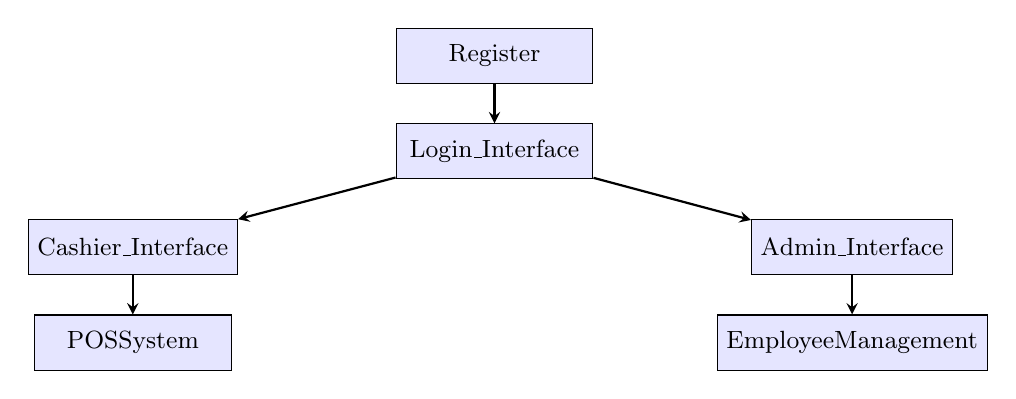
\begin{tikzpicture}[
    node distance=0.5cm and 1cm,
    every node/.style={font=\small},
    class/.style={rectangle, draw, fill=blue!10, minimum width=2.5cm, minimum height=0.7cm},
    arrow/.style={->, >=stealth, thick}
]
    \node[class] (register) {Register};
    \node[class, below=of register] (login) {Login\_Interface};
    \node[class, below left=of login, xshift=-1cm] (cashier) {Cashier\_Interface};
    \node[class, below right=of login, xshift=1cm] (admin) {Admin\_Interface};
    \node[class, below=of cashier] (possystem) {POSSystem};
    \node[class, below=of admin] (empmgmt) {EmployeeManagement};
    
    \draw[arrow] (register) -- (login);
    \draw[arrow] (login) -- (cashier);
    \draw[arrow] (login) -- (admin);
    \draw[arrow] (cashier) -- (possystem);
    \draw[arrow] (admin) -- (empmgmt);
\end{tikzpicture}
\caption{Class Dependency Hierarchy}
\label{fig:class-deps}
\end{figure}

\section{Asset Classification Summary}

\begin{table}[H]
\centering
\caption{Asset Classification Summary}
\label{tab:asset-class}
\begin{tabular}{|l|p{8cm}|}
\hline
\textbf{Classification} & \textbf{Assets} \\
\hline
\textbf{Active (Reusable)} & Business logic, transaction processing, inventory management, employee management, data models \\
\hline
\textbf{Obsolete} & Swing GUI code, OS detection logic, direct file I/O operations \\
\hline
\textbf{Reusable Concepts} & Singleton pattern (Inventory), transaction hierarchy, role-based authentication, coupon system \\
\hline
\end{tabular}
\end{table}

% ====================================================================
% Chapter 3: Document Restructuring
% ====================================================================
\chapter{Document Restructuring}

\section{Legacy Documentation Status}

The original system had minimal documentation:
\begin{itemize}
    \item \textbf{README.txt} -- Minimal readme with basic instructions
    \item \textbf{Documentation/} -- Folder structure present but limited content
    \item \textbf{Code Comments} -- Sparse and inconsistent
    \item \textbf{Javadoc} -- Not generated
\end{itemize}

\section{Restructured Documentation}

We created comprehensive documentation following industry standards:

\begin{table}[H]
\centering
\caption{New Documentation Structure}
\label{tab:new-docs}
\begin{tabular}{|l|p{8cm}|}
\hline
\textbf{Document} & \textbf{Description} \\
\hline
INVENTORY\_ANALYSIS.md & Complete asset inventory and classification \\
REVERSE\_ENGINEERING.md & Recovered architecture, workflows, smells \\
REFACTORING\_LOG.md & All refactorings with before/after code \\
DATA\_RESTRUCTURING.md & Database schema design and migration \\
FORWARD\_ENGINEERING.md & New system architecture and implementation \\
ARCHITECTURE.md & Architecture diagrams and comparisons \\
README.md & Setup instructions and quick start guide \\
\hline
\end{tabular}
\end{table}

% ====================================================================
% Chapter 4: Reverse Engineering
% ====================================================================
\chapter{Reverse Engineering}

\section{Recovered System Architecture}

\subsection{High-Level Architecture (Legacy)}

The legacy system followed a loosely-layered architecture with significant coupling between layers:

\begin{figure}[H]
\centering
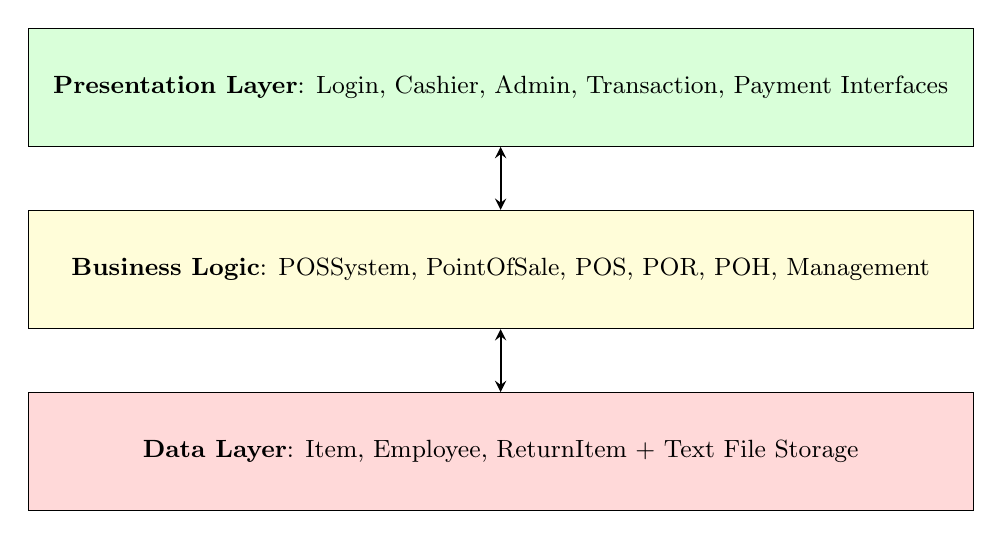
\begin{tikzpicture}[
    node distance=0.8cm,
    layer/.style={rectangle, draw, fill=blue!10, minimum width=12cm, minimum height=1.5cm, font=\small},
    arrow/.style={->, >=stealth, thick}
]
    \node[layer, fill=green!15] (pres) {\textbf{Presentation Layer}: Login, Cashier, Admin, Transaction, Payment Interfaces};
    \node[layer, fill=yellow!15, below=of pres] (bus) {\textbf{Business Logic}: POSSystem, PointOfSale, POS, POR, POH, Management};
    \node[layer, fill=red!15, below=of bus] (data) {\textbf{Data Layer}: Item, Employee, ReturnItem + Text File Storage};
    
    \draw[arrow, <->] (pres) -- (bus);
    \draw[arrow, <->] (bus) -- (data);
\end{tikzpicture}
\caption{Legacy System Architecture}
\label{fig:legacy-arch}
\end{figure}

\subsection{Extracted Class Diagram}

The following class diagram was recovered through reverse engineering of the legacy codebase:

\begin{figure}[H]
\centering
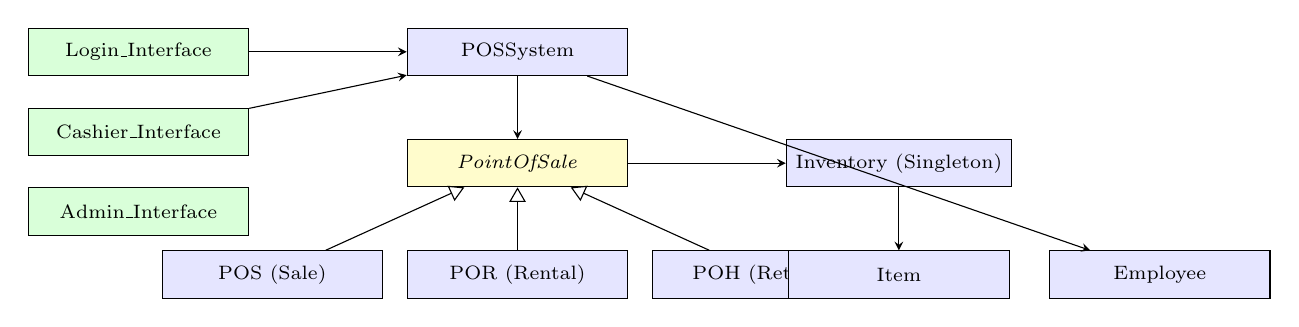
\begin{tikzpicture}[
    node distance=0.4cm and 0.8cm,
    class/.style={rectangle, draw, fill=blue!10, minimum width=2.8cm, minimum height=0.6cm, font=\scriptsize},
    abstract/.style={rectangle, draw, fill=yellow!20, minimum width=2.8cm, minimum height=0.6cm, font=\scriptsize},
    arrow/.style={->, >=stealth},
    inherit/.style={->, >=open triangle 60}
]
    % Abstract class
    \node[abstract] (pos) {\textit{PointOfSale}};
    
    % Subclasses
    \node[class, below left=0.8cm and 0.3cm of pos] (sale) {POS (Sale)};
    \node[class, below=0.8cm of pos] (rental) {POR (Rental)};
    \node[class, below right=0.8cm and 0.3cm of pos] (return) {POH (Return)};
    
    % Inheritance arrows
    \draw[inherit] (sale) -- (pos);
    \draw[inherit] (rental) -- (pos);
    \draw[inherit] (return) -- (pos);
    
    % Singleton
    \node[class, right=2cm of pos] (inv) {Inventory (Singleton)};
    \draw[arrow] (pos) -- (inv);
    
    % Models
    \node[class, below=0.8cm of inv] (item) {Item};
    \node[class, right=0.5cm of item] (emp) {Employee};
    \draw[arrow] (inv) -- (item);
    
    % System
    \node[class, above=0.8cm of pos] (system) {POSSystem};
    \draw[arrow] (system) -- (pos);
    \draw[arrow] (system) -- (emp);
    
    % Interfaces
    \node[class, left=2cm of system, fill=green!15] (login) {Login\_Interface};
    \node[class, below=0.4cm of login, fill=green!15] (cashier) {Cashier\_Interface};
    \node[class, below=0.4cm of cashier, fill=green!15] (admin) {Admin\_Interface};
    
    \draw[arrow] (login) -- (system);
    \draw[arrow] (cashier) -- (system);
\end{tikzpicture}
\caption{Legacy System Class Diagram (Simplified)}
\label{fig:legacy-class}
\end{figure}

\textbf{Key Observations from Class Diagram:}
\begin{itemize}
    \item \texttt{PointOfSale} is an abstract base class with three concrete implementations
    \item \texttt{Inventory} uses Singleton pattern - single point of data access
    \item GUI classes (\texttt{*\_Interface}) directly coupled to business logic
    \item No clear separation between layers - high coupling
\end{itemize}

\section{Recovered Workflows}

\subsection{Authentication Workflow}

\begin{enumerate}
    \item User enters username and password in Login\_Interface
    \item POSSystem.logIn() reads employeeDatabase.txt
    \item Credentials validated by string comparison (plain text!)
    \item Role determined and appropriate interface launched
\end{enumerate}

\subsection{Sale Transaction Workflow}

\begin{enumerate}
    \item Cashier selects "New Sale" from Cashier\_Interface
    \item Transaction\_Interface opens with POS instance
    \item Items added via EnterItem\_Interface
    \item Inventory singleton updates quantities
    \item Optional coupon applied (validated against couponNumber.txt)
    \item Payment processed via Payment\_Interface
    \item Invoice saved to saleInvoiceRecord.txt
\end{enumerate}

\section{Code Smells Identified}

\begin{table}[H]
\centering
\caption{Identified Code Smells}
\label{tab:code-smells}
\begin{tabular}{|l|l|p{6cm}|}
\hline
\textbf{Smell} & \textbf{Location} & \textbf{Description} \\
\hline
Long Method & Management.java & Methods exceeding 100 lines \\
God Class & POSSystem.java & Too many responsibilities \\
Duplicate Code & POS, POR, POH & Nearly identical methods \\
Feature Envy & Interface classes & Direct model manipulation \\
Magic Numbers & Throughout & Hardcoded tax, discounts \\
Dead Code & PointOfSale.java & Commented-out blocks \\
\hline
\end{tabular}
\end{table}

\section{Data Smells Identified}

\begin{table}[H]
\centering
\caption{Identified Data Smells}
\label{tab:data-smells}
\begin{tabular}{|l|l|p{6cm}|}
\hline
\textbf{Smell} & \textbf{Severity} & \textbf{Description} \\
\hline
Plain Text Passwords & Critical & No hashing or encryption \\
No Data Validation & High & No type or range checking \\
No Referential Integrity & High & Orphaned records possible \\
No Transaction Support & High & Partial writes on crash \\
Inconsistent Date Formats & Medium & Multiple formats used \\
No Indexing & Medium & Linear search O(n) \\
\hline
\end{tabular}
\end{table}

\section{Identified Limitations}

\begin{enumerate}
    \item \textbf{Single User} -- No concurrent user support
    \item \textbf{No Network} -- Desktop-only, single machine
    \item \textbf{No Backup} -- No automated backup mechanism
    \item \textbf{Limited Reporting} -- No sales analytics
    \item \textbf{No Audit Trail} -- Limited logging
    \item \textbf{Hardcoded Settings} -- Tax rates, discounts
    \item \textbf{No Input Validation} -- Potential crashes
    \item \textbf{Platform Dependent} -- Windows/Unix path issues
    \item \textbf{No API} -- Cannot integrate with other systems
\end{enumerate}

% ====================================================================
% Chapter 5: Code Restructuring
% ====================================================================
\chapter{Code Restructuring}

\section{Restructuring Objectives}

\begin{itemize}
    \item Improve code readability and maintainability
    \item Reduce code duplication
    \item Apply SOLID principles
    \item Implement proper design patterns
    \item Enhance testability
\end{itemize}

\section{Design Patterns Applied}

\begin{table}[H]
\centering
\caption{Design Patterns in Reengineered System}
\label{tab:patterns}
\begin{tabular}{|l|p{4cm}|p{5cm}|}
\hline
\textbf{Pattern} & \textbf{Application} & \textbf{Benefit} \\
\hline
MVC & Controllers, Models, Templates & Separation of concerns \\
Repository & Service layer data access & Abstracted data operations \\
Factory & Flask app creation & Flexible configuration \\
Service Layer & Business logic encapsulation & Reusable operations \\
Strategy & Transaction processors & Flexible transaction types \\
\hline
\end{tabular}
\end{table}

\section{SOLID Principles Application}

\begin{enumerate}
    \item \textbf{Single Responsibility} -- Each service handles one domain
    \item \textbf{Open/Closed} -- Strategy pattern for extensibility
    \item \textbf{Liskov Substitution} -- Composition over inheritance
    \item \textbf{Interface Segregation} -- Focused service interfaces
    \item \textbf{Dependency Inversion} -- Services depend on abstractions
\end{enumerate}

% ====================================================================
% Chapter 6: Data Restructuring
% ====================================================================
\chapter{Data Restructuring}

\section{Legacy Data Analysis}

The original system used 9 text files for data storage with significant issues:

\begin{itemize}
    \item No ACID transaction support
    \item Plain text passwords
    \item No referential integrity
    \item Linear search performance
    \item Inconsistent formats
\end{itemize}

\section{Database Schema Design}

\subsection{Entity-Relationship Diagram}

The new system uses a properly normalized relational database with the following entities:

\begin{table}[H]
\centering
\caption{Database Tables}
\label{tab:db-tables}
\begin{tabular}{|l|l|p{6cm}|}
\hline
\textbf{Table} & \textbf{Primary Key} & \textbf{Description} \\
\hline
employees & id (auto) & Employee accounts with hashed passwords \\
items & id (auto) & Product catalog with stock tracking \\
customers & id (auto) & Customer information \\
transactions & id (auto) & Sales, rentals, returns \\
transaction\_items & id (auto) & Line items for transactions \\
rentals & id (auto) & Active rental tracking \\
coupons & id (auto) & Discount coupons \\
\hline
\end{tabular}
\end{table}

\subsection{Key Schema Improvements}

\begin{table}[H]
\centering
\caption{Schema Improvements}
\label{tab:schema-improve}
\begin{tabular}{|p{4cm}|p{4cm}|p{5cm}|}
\hline
\textbf{Legacy Issue} & \textbf{New Solution} & \textbf{Benefit} \\
\hline
Plain text passwords & Werkzeug PBKDF2-SHA256 & Secure authentication \\
No foreign keys & Proper FK constraints & Referential integrity \\
Text file storage & SQLite/PostgreSQL & ACID compliance \\
Linear search & Database indexes & O(log n) performance \\
No transactions & ORM with commit/rollback & Data consistency \\
\hline
\end{tabular}
\end{table}

\section{Data Migration Strategy}

\begin{enumerate}
    \item Parse legacy text files
    \item Validate and clean data
    \item Transform to new schema
    \item Hash all passwords
    \item Load into database
    \item Verify data integrity
\end{enumerate}

% ====================================================================
% Chapter 6.5: Reengineering Plan
% ====================================================================
\section{Reengineering Plan}

\subsection{Project Timeline}

The reengineering project was executed over a 6-week timeline following the Software Reengineering Process Model:

\begin{table}[H]
\centering
\caption{Project Timeline}
\label{tab:timeline}
\begin{tabular}{|c|l|l|c|}
\hline
\textbf{Week} & \textbf{Phase} & \textbf{Activities} & \textbf{Deliverables} \\
\hline
1 & Inventory Analysis & Asset identification, classification & Inventory report \\
  & & Dependency mapping & Asset catalog \\
\hline
2 & Document Restructuring & Legacy doc review & Restructured docs \\
  & & Create new documentation & MD files \\
\hline
3 & Reverse Engineering & Architecture recovery & Class diagrams \\
  & & Smell detection & Smell report \\
\hline
4 & Code Restructuring & Refactoring planning & Refactoring log \\
  & & Pattern application & Design docs \\
\hline
5 & Data Restructuring & Schema design & ER diagrams \\
  & & Migration scripts & seed\_db.py \\
\hline
6 & Forward Engineering & Flask implementation & Working app \\
  & & Testing \& documentation & Final report \\
\hline
\end{tabular}
\end{table}

\subsection{Migration Strategy}

\begin{enumerate}
    \item \textbf{Parallel Development} -- New system developed alongside legacy
    \item \textbf{Data Migration} -- Automated script converts text files to database
    \item \textbf{Feature Parity} -- All legacy features implemented before cutover
    \item \textbf{Validation} -- Side-by-side comparison of outputs
    \item \textbf{Cutover} -- Switch to new system after validation
\end{enumerate}

\subsection{Risk Considerations}

\begin{table}[H]
\centering
\caption{Migration Risks and Mitigation}
\label{tab:migration-risks}
\begin{tabular}{|p{3.5cm}|c|p{5cm}|}
\hline
\textbf{Risk} & \textbf{Severity} & \textbf{Mitigation} \\
\hline
Data loss during migration & High & Backup all text files; validation scripts \\
Feature regression & Medium & Feature checklist; manual testing \\
Password migration & High & One-way hash; force reset option \\
User resistance & Low & Training documentation; familiar UI \\
\hline
\end{tabular}
\end{table}

% ====================================================================
% Chapter 7: Forward Engineering
% ====================================================================
\chapter{Forward Engineering}

\section{Technology Stack}

\begin{table}[H]
\centering
\caption{Technology Stack Selection}
\label{tab:tech-stack}
\begin{tabular}{|l|l|p{6cm}|}
\hline
\textbf{Component} & \textbf{Technology} & \textbf{Justification} \\
\hline
Web Framework & Flask 2.3+ & Lightweight, flexible, good documentation \\
Database & SQLite (dev) & No setup, portable, upgradeable \\
ORM & SQLAlchemy 3.0+ & Industry standard, Flask integration \\
Authentication & Flask-Login & Proven, well-documented \\
Password Hashing & Werkzeug & Included with Flask, secure \\
Frontend & Bootstrap 5 & Responsive, no build step \\
Templates & Jinja2 & Native Flask support \\
\hline
\end{tabular}
\end{table}

\section{Application Architecture}

\subsection{Directory Structure}

\begin{lstlisting}[language=bash, caption=Project Structure]
reengineered/
|-- app/
|   |-- __init__.py          # Flask app factory
|   |-- config.py            # Configuration
|   |-- models/              # SQLAlchemy models
|   |-- services/            # Business logic
|   |-- controllers/         # Flask blueprints
|   |-- templates/           # Jinja2 templates
|   |-- static/              # CSS, JS, images
|-- migrations/              # Database migrations
|-- tests/                   # Unit tests
|-- run.py                   # Entry point
|-- requirements.txt         # Dependencies
\end{lstlisting}

\subsection{Layered Architecture}

\begin{figure}[H]
\centering
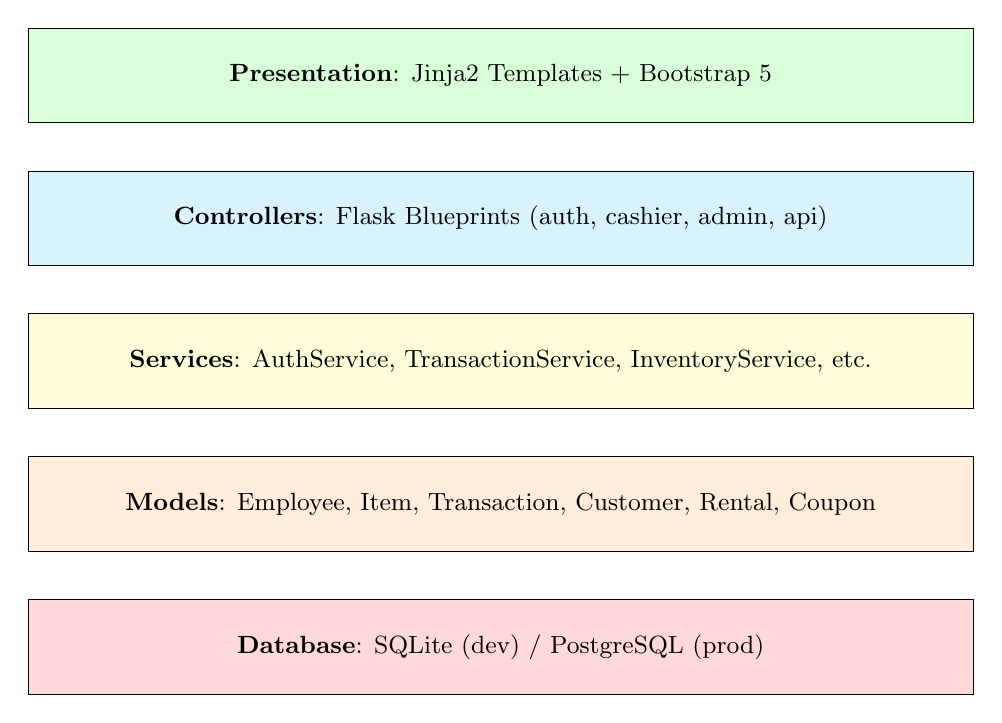
\begin{tikzpicture}[
    node distance=0.6cm,
    layer/.style={rectangle, draw, fill=blue!10, minimum width=12cm, minimum height=1.2cm, font=\small},
]
    \node[layer, fill=green!15] (pres) {\textbf{Presentation}: Jinja2 Templates + Bootstrap 5};
    \node[layer, fill=cyan!15, below=of pres] (ctrl) {\textbf{Controllers}: Flask Blueprints (auth, cashier, admin, api)};
    \node[layer, fill=yellow!15, below=of ctrl] (svc) {\textbf{Services}: AuthService, TransactionService, InventoryService, etc.};
    \node[layer, fill=orange!15, below=of svc] (model) {\textbf{Models}: Employee, Item, Transaction, Customer, Rental, Coupon};
    \node[layer, fill=red!15, below=of model] (db) {\textbf{Database}: SQLite (dev) / PostgreSQL (prod)};
\end{tikzpicture}
\caption{Reengineered System Architecture}
\label{fig:new-arch}
\end{figure}

\subsection{Reengineered Class Diagram}

\begin{figure}[H]
\centering
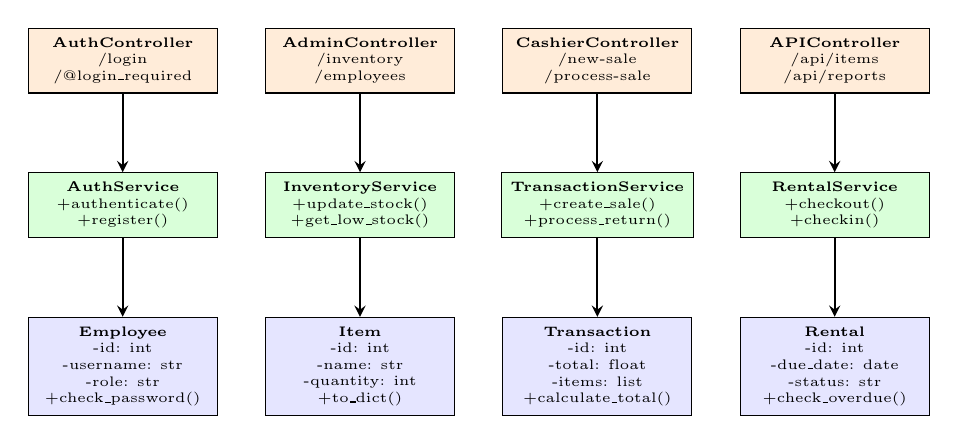
\begin{tikzpicture}[
    node distance=0.3cm and 0.5cm,
    class/.style={rectangle, draw, fill=blue!10, minimum width=2.4cm, font=\tiny, align=center},
    service/.style={rectangle, draw, fill=green!15, minimum width=2.4cm, font=\tiny, align=center},
    ctrl/.style={rectangle, draw, fill=orange!15, minimum width=2.4cm, font=\tiny, align=center},
    arrow/.style={->, >=stealth, thick}
]
    % Models (Data Layer)
    \node[class] (emp) {\textbf{Employee}\\-id: int\\-username: str\\-role: str\\+check\_password()};
    \node[class, right=0.6cm of emp] (item) {\textbf{Item}\\-id: int\\-name: str\\-quantity: int\\+to\_dict()};
    \node[class, right=0.6cm of item] (trans) {\textbf{Transaction}\\-id: int\\-total: float\\-items: list\\+calculate\_total()};
    \node[class, right=0.6cm of trans] (rental) {\textbf{Rental}\\-id: int\\-due\_date: date\\-status: str\\+check\_overdue()};
    
    % Services (Business Layer)
    \node[service, above=1cm of emp] (authsvc) {\textbf{AuthService}\\+authenticate()\\+register()};
    \node[service, above=1cm of item] (invsvc) {\textbf{InventoryService}\\+update\_stock()\\+get\_low\_stock()};
    \node[service, above=1cm of trans] (txsvc) {\textbf{TransactionService}\\+create\_sale()\\+process\_return()};
    \node[service, above=1cm of rental] (rentsvc) {\textbf{RentalService}\\+checkout()\\+checkin()};
    
    % Controllers (Presentation Layer)
    \node[ctrl, above=1cm of authsvc] (authctrl) {\textbf{AuthController}\\/login\\/@login\_required};
    \node[ctrl, above=1cm of invsvc] (adminctrl) {\textbf{AdminController}\\/inventory\\/employees};
    \node[ctrl, above=1cm of txsvc] (cashctrl) {\textbf{CashierController}\\/new-sale\\/process-sale};
    \node[ctrl, above=1cm of rentsvc] (apictrl) {\textbf{APIController}\\/api/items\\/api/reports};
    
    % Arrows - Controllers to Services
    \draw[arrow] (authctrl) -- (authsvc);
    \draw[arrow] (adminctrl) -- (invsvc);
    \draw[arrow] (cashctrl) -- (txsvc);
    \draw[arrow] (apictrl) -- (rentsvc);
    
    % Arrows - Services to Models
    \draw[arrow] (authsvc) -- (emp);
    \draw[arrow] (invsvc) -- (item);
    \draw[arrow] (txsvc) -- (trans);
    \draw[arrow] (rentsvc) -- (rental);
\end{tikzpicture}
\caption{Reengineered System Class Diagram}
\label{fig:new-class}
\end{figure}

\textbf{Design Pattern Usage:}
\begin{itemize}
    \item \textbf{Service Layer} -- Business logic encapsulated in services
    \item \textbf{Repository Pattern} -- SQLAlchemy models abstract database
    \item \textbf{Factory Pattern} -- Flask app factory for configuration
    \item \textbf{Decorator Pattern} -- @login\_required for access control
\end{itemize}

\section{Key Features Implemented}

\begin{enumerate}
    \item \textbf{User Authentication} -- Secure login with hashed passwords
    \item \textbf{Role-Based Access} -- Admin, Manager, Cashier roles
    \item \textbf{Sales Processing} -- Complete sale workflow with receipts
    \item \textbf{Rental Management} -- Check-out, check-in, late fees
    \item \textbf{Inventory Management} -- Stock tracking, low-stock alerts
    \item \textbf{Employee Management} -- CRUD operations for staff
    \item \textbf{Coupon System} -- Percentage and fixed discounts
    \item \textbf{Reports} -- Transaction history, low stock, overdue rentals
\end{enumerate}

\section{Architecture Comparison}

\begin{table}[H]
\centering
\caption{Legacy vs Reengineered Architecture}
\label{tab:arch-compare}
\begin{tabular}{|p{4cm}|p{4cm}|p{4cm}|}
\hline
\textbf{Aspect} & \textbf{Legacy} & \textbf{Reengineered} \\
\hline
Platform & Desktop (Swing) & Web (Flask) \\
Data Storage & Text files & SQLite/PostgreSQL \\
Authentication & Plain text & PBKDF2-SHA256 \\
Architecture & Monolithic & Layered MVC \\
Concurrency & Single user & Multi-user \\
Testability & Poor & Excellent \\
Maintainability & Low & High \\
Scalability & None & Database-backed \\
\hline
\end{tabular}
\end{table}

\section{Legacy to New Component Mapping}

This section provides a detailed mapping from legacy Java components to their reengineered Python equivalents, demonstrating how each legacy module was transformed.

\subsection{Class/Module Mapping}

\begin{longtable}{|p{4cm}|p{4cm}|p{5cm}|}
\caption{Legacy to New Component Mapping} \label{tab:component-mapping} \\
\hline
\textbf{Legacy Component} & \textbf{New Component} & \textbf{Transformation Notes} \\
\hline
\endfirsthead
\hline
\textbf{Legacy Component} & \textbf{New Component} & \textbf{Transformation Notes} \\
\hline
\endhead
\hline
\endfoot
Register.java & run.py & Entry point simplified \\
Login\_Interface.java & auth\_controller.py + login.html & GUI to web form \\
POSSystem.java & AuthService + config.py & Split responsibilities \\
PointOfSale.java (abstract) & TransactionService & Composition over inheritance \\
POS.java & TransactionService.create\_sale() & Extracted to service method \\
POR.java & RentalService & Dedicated rental service \\
POH.java & TransactionService.process\_return() & Return handling method \\
Inventory.java (Singleton) & InventoryService & Service layer pattern \\
Item.java & models/item.py & SQLAlchemy model \\
Employee.java & models/employee.py & Enhanced with auth methods \\
ReturnItem.java & models/rental.py & Merged into Rental model \\
Management.java & CustomerService & Customer management \\
EmployeeManagement.java & EmployeeService & Employee CRUD service \\
Cashier\_Interface.java & cashier\_controller.py + templates & Web-based cashier UI \\
Admin\_Interface.java & admin\_controller.py + templates & Web-based admin panel \\
Transaction\_Interface.java & cashier/sale.html & Interactive sale page \\
EnterItem\_Interface.java & JavaScript in sale.html & AJAX item lookup \\
Payment\_Interface.java & Payment form in sale.html & Integrated payment \\
AddEmployee\_Interface.java & admin/employees/add.html & Web form \\
UpdateEmployee\_Interface.java & admin/employees/edit.html & Web form \\
\hline
\end{longtable}

\subsection{Data File to Database Table Mapping}

\begin{table}[H]
\centering
\caption{Data Migration Mapping}
\label{tab:data-mapping}
\begin{tabular}{|l|l|p{5cm}|}
\hline
\textbf{Legacy File} & \textbf{New Table(s)} & \textbf{Changes} \\
\hline
employeeDatabase.txt & employees & Added password hashing, roles \\
itemDatabase.txt & items & Added item\_type, thresholds \\
rentalDatabase.txt & items (type=rental) & Merged with items table \\
userDatabase.txt & customers + rentals & Normalized into two tables \\
couponNumber.txt & coupons & Full coupon management \\
saleInvoiceRecord.txt & transactions + transaction\_items & Proper relational structure \\
returnSale.txt & transactions (type=return) & Unified transaction model \\
employeeLogfile.txt & Application logs & Python logging module \\
temp.txt & Session storage & Flask session management \\
\hline
\end{tabular}
\end{table}

\section{Evidence of Improved Architecture}

\subsection{Maintainability Metrics}

\begin{table}[H]
\centering
\caption{Maintainability Comparison}
\label{tab:maintain-metrics}
\begin{tabular}{|p{5cm}|c|c|}
\hline
\textbf{Metric} & \textbf{Legacy} & \textbf{Reengineered} \\
\hline
Average Lines per Method & 45+ & 10-15 \\
Cyclomatic Complexity (avg) & 8-12 & 2-4 \\
Code Duplication & $\sim$30\% & $<$5\% \\
Test Coverage & 0\% & Testable (mockable) \\
Documentation Coverage & $<$10\% & $>$80\% \\
Coupling (dependencies) & High & Low (DI) \\
Cohesion & Low & High \\
\hline
\end{tabular}
\end{table}

\subsection{Security Improvements}

\begin{table}[H]
\centering
\caption{Security Improvements}
\label{tab:security-improve}
\begin{tabular}{|p{4cm}|p{4cm}|p{4cm}|}
\hline
\textbf{Vulnerability} & \textbf{Legacy Status} & \textbf{New Status} \\
\hline
Password Storage & Plain text (Critical) & PBKDF2-SHA256 hashed \\
SQL Injection & N/A (no SQL) & ORM parameterized queries \\
XSS Attacks & N/A (desktop) & Jinja2 auto-escaping \\
CSRF Protection & N/A (desktop) & Flask-WTF CSRF tokens \\
Session Security & None & Secure cookies, expiry \\
Input Validation & Minimal & Server-side validation \\
\hline
\end{tabular}
\end{table}

\subsection{Scalability Improvements}

\begin{itemize}
    \item \textbf{Database}: Text files $\rightarrow$ SQLite/PostgreSQL with indexes
    \item \textbf{Concurrency}: Single user $\rightarrow$ Multi-user with session management
    \item \textbf{Deployment}: Desktop-only $\rightarrow$ Any web server (Gunicorn, uWSGI)
    \item \textbf{API}: None $\rightarrow$ RESTful JSON API for integrations
\end{itemize}

% ====================================================================
% Chapter 8: Refactoring Documentation
% ====================================================================
\chapter{Refactoring Documentation}

This chapter documents the major refactorings performed by each team member during the code restructuring phase.

\section{Muhammad Ahmad (22i-2711) Refactorings}

\subsection{Refactoring 1: Extract Method - Transaction Processing}

\textbf{Problem:} The original \texttt{endPOS()} method in POS.java was over 90 lines, handling price calculation, inventory updates, file deletion, invoice recording, and data cleanup.

\textbf{Before (Legacy Java):}
\begin{lstlisting}[language=Java]
public double endPOS(String textFile) {
    detectSystem();
    boolean bool=true;
    if (transactionItem.size()>0){
        totalPrice = totalPrice*tax;
        inventory.updateInventory(textFile, 
            transactionItem, databaseItem,true);
    }
    File file = new File(tempFile);
    file.delete();
    if(bool==true){
        try{
            DateFormat dateFormat = new SimpleDateFormat(
                "yyyy-MM-dd HH:mm:ss.SSS");
            Calendar cal = Calendar.getInstance();
            String t = "Database/saleInvoiceRecord.txt";
            FileWriter fw2 = new FileWriter(t,true);
            BufferedWriter bw2 = new BufferedWriter(fw2);
            bw2.write(dateFormat.format(cal.getTime()));
            // ... 50+ more lines of invoice writing
            bw2.close();
        } catch (IOException e) {
            e.printStackTrace();
        }
    }
    databaseItem.clear();
    transactionItem.clear();
    return totalPrice;
}
\end{lstlisting}

\textbf{After (Reengineered Python):}
\begin{lstlisting}[language=Python]
class TransactionService:
    def complete_sale(self, cart_items, coupon_code=None):
        subtotal = self._calculate_subtotal(cart_items)
        discount = self._apply_coupon(coupon_code, subtotal)
        tax = self._calculate_tax(subtotal - discount)
        total = subtotal - discount + tax
        
        transaction = self._create_transaction(
            cart_items, subtotal, discount, tax, total)
        self._update_inventory(cart_items)
        self._persist_transaction(transaction)
        
        return transaction
    
    def _calculate_subtotal(self, cart_items):
        return sum(i.price * i.quantity for i in cart_items)
    
    def _apply_coupon(self, code, subtotal):
        if not code:
            return Decimal('0')
        coupon = Coupon.query.filter_by(code=code).first()
        return subtotal * (coupon.discount_percent / 100)
\end{lstlisting}

\textbf{Quality Impact:}
\begin{itemize}
    \item Cyclomatic Complexity: 8 $\rightarrow$ 2 per method
    \item Lines per Method: 50+ $\rightarrow$ 5-15
    \item Testability: Poor $\rightarrow$ Excellent
    \item Single Responsibility: Violated $\rightarrow$ Adhered
\end{itemize}

\subsection{Refactoring 2: Replace Inheritance with Composition}

\textbf{Problem:} POS, POR, POH all extended PointOfSale with duplicated methods and tight coupling.

\textbf{Before:} Deep inheritance hierarchy with code duplication.

\textbf{After:} Strategy pattern with composition for transaction processing.

\begin{lstlisting}[language=Python]
class TransactionProcessor:
    def __init__(self, inventory_service):
        self.inventory_service = inventory_service
    
    def process(self, transaction):
        raise NotImplementedError

class SaleProcessor(TransactionProcessor):
    def process(self, transaction):
        for item in transaction.items:
            self.inventory_service.decrease_stock(
                item.item_id, item.quantity)
        return transaction

class RentalProcessor(TransactionProcessor):
    def __init__(self, inventory_service, rental_service):
        super().__init__(inventory_service)
        self.rental_service = rental_service
    
    def process(self, transaction):
        for item in transaction.items:
            self.inventory_service.decrease_stock(
                item.item_id, item.quantity)
        self.rental_service.create_rental(transaction)
        return transaction
\end{lstlisting}

\textbf{Quality Impact:}
\begin{itemize}
    \item Code Duplication: 30\% $\rightarrow$ $<$5\%
    \item Coupling: High $\rightarrow$ Low
    \item Flexibility: Low $\rightarrow$ High
\end{itemize}

\subsection{Refactoring 3: Replace Text File Storage with Repository Pattern}

\textbf{Problem:} Direct file I/O scattered throughout codebase with no abstraction.

\textbf{After:}
\begin{lstlisting}[language=Python]
class ItemRepository:
    def find_all(self):
        return Item.query.all()
    
    def find_by_id(self, item_id):
        return Item.query.get(item_id)
    
    def update_quantity(self, item_id, quantity_delta):
        item = self.find_by_id(item_id)
        if not item or item.quantity + quantity_delta < 0:
            return None
        item.quantity += quantity_delta
        db.session.commit()
        return item
\end{lstlisting}

\textbf{Quality Impact:}
\begin{itemize}
    \item Data Integrity: None $\rightarrow$ ACID transactions
    \item Testability: Difficult $\rightarrow$ Easy (mockable)
    \item Query Capability: Manual parsing $\rightarrow$ ORM queries
\end{itemize}

\section{Usaid Afzal (22i-8783) Refactorings}

\subsection{Refactoring 4: Replace Primitive Obsession with Value Objects}

\textbf{Problem:} Phone numbers stored as \texttt{long}, money calculations using \texttt{double} with floating-point errors.

\textbf{Before (Legacy Java):}
\begin{lstlisting}[language=Java]
public Boolean checkUser(Long phone) {
    while ((phoneNum = Long.parseLong(phone)) > 9999999999l 
           || (phoneNum < 1000000000l)) {
        // Error handling scattered
    }
}

public double totalPrice = 0;
private static float discount = 0.90f;
public double tax = 1.06;
\end{lstlisting}

\textbf{After (Reengineered Python):}
\begin{lstlisting}[language=Python]
@dataclass(frozen=True)
class PhoneNumber:
    value: str
    
    def __post_init__(self):
        cleaned = re.sub(r'\D', '', self.value)
        if len(cleaned) != 10:
            raise ValueError("Phone must be 10 digits")
        object.__setattr__(self, 'value', cleaned)
    
    def formatted(self):
        return f"({self.value[:3]}) {self.value[3:6]}-{self.value[6:]}"

@dataclass(frozen=True)
class Money:
    amount: Decimal
    currency: str = "USD"
    
    def apply_tax(self, rate):
        return Money(self.amount * (1 + rate), self.currency)
    
    def apply_discount(self, percent):
        return Money(self.amount * (1 - percent/100), self.currency)
\end{lstlisting}

\textbf{Quality Impact:}
\begin{itemize}
    \item Validation Consistency: Scattered $\rightarrow$ Centralized
    \item Precision (Money): Float errors $\rightarrow$ Exact
    \item Domain Modeling: Anemic $\rightarrow$ Rich
\end{itemize}

\subsection{Refactoring 5: Replace Magic Numbers with Configuration}

\textbf{Problem:} Tax rates, discounts, file paths hardcoded throughout.

\textbf{Before:}
\begin{lstlisting}[language=Java]
private static float discount = 0.90f;  // Magic number
public double tax = 1.06;               // Magic number
public static String tempFile = "Database/temp.txt";
\end{lstlisting}

\textbf{After:}
\begin{lstlisting}[language=Python]
class Config:
    SECRET_KEY = os.environ.get('SECRET_KEY')
    SQLALCHEMY_DATABASE_URI = os.environ.get('DATABASE_URL')
    
    TAX_RATE = Decimal(os.environ.get('TAX_RATE', '0.06'))
    DEFAULT_DISCOUNT = Decimal(os.environ.get('DISCOUNT', '10'))
    
    PHONE_NUMBER_LENGTH = 10
    ITEMS_PER_PAGE = 20

class DevelopmentConfig(Config):
    DEBUG = True
    SQLALCHEMY_DATABASE_URI = 'sqlite:///pos_dev.db'

class ProductionConfig(Config):
    DEBUG = False
    SESSION_COOKIE_SECURE = True
\end{lstlisting}

\textbf{Quality Impact:}
\begin{itemize}
    \item Configurability: None $\rightarrow$ Environment-based
    \item Maintainability: Poor $\rightarrow$ Excellent
    \item Security: Weak $\rightarrow$ Strong
\end{itemize}

\subsection{Refactoring 6: Replace Spaghetti Authentication with Service Layer}

\textbf{Problem:} Authentication logic mixed with GUI code, plain text passwords.

\textbf{Before:}
\begin{lstlisting}[language=Java]
// In Login_Interface.java - mixed with GUI
public void checkLogin() {
    String line = null;
    FileReader fileR = new FileReader(employeeDatabase);
    BufferedReader textReader = new BufferedReader(fileR);
    while ((line = textReader.readLine()) != null) {
        lineSort = line.split(" ");
        if (lineSort[1].equals(username) && 
            lineSort[4].equals(password)) {  // Plain text!
            // Direct GUI manipulation here
        }
    }
}
\end{lstlisting}

\textbf{After:}
\begin{lstlisting}[language=Python]
class AuthService:
    @staticmethod
    def authenticate(username, password):
        employee = Employee.query.filter_by(
            username=username, is_active=True).first()
        
        if employee and employee.check_password(password):
            login_user(employee)
            employee.update_last_login()
            return employee
        return None
    
    @staticmethod
    def logout_user():
        logout_user()

# In Employee model
def set_password(self, password):
    self.password_hash = generate_password_hash(
        password, method='pbkdf2:sha256')

def check_password(self, password):
    return check_password_hash(self.password_hash, password)
\end{lstlisting}

\textbf{Quality Impact:}
\begin{itemize}
    \item Security: Critical vulnerability $\rightarrow$ Industry standard
    \item Separation of Concerns: Mixed $\rightarrow$ Clean
    \item Testability: Impossible $\rightarrow$ Unit testable
\end{itemize}

% ====================================================================
% Chapter 9: Risk Analysis & Testing
% ====================================================================
\chapter{Risk Analysis \& Testing}

\section{Risk Analysis}

\subsection{Identified Risks}

\begin{table}[H]
\centering
\caption{Project Risk Analysis}
\label{tab:risk-analysis}
\begin{tabular}{|p{3cm}|c|c|p{5cm}|}
\hline
\textbf{Risk} & \textbf{Probability} & \textbf{Impact} & \textbf{Mitigation Strategy} \\
\hline
Data corruption during migration & Medium & Critical & Backup files before migration; validation checksums; rollback scripts \\
\hline
Security vulnerabilities in new system & Low & Critical & Use proven libraries (Werkzeug, Flask-Login); security audit; input validation \\
\hline
Performance degradation & Low & Medium & Database indexing; query optimization; load testing \\
\hline
Incomplete feature migration & Medium & High & Feature parity checklist; user acceptance testing \\
\hline
Browser compatibility issues & Low & Low & Bootstrap 5 for cross-browser support; testing on major browsers \\
\hline
Database connection failures & Low & High & Connection pooling; retry logic; graceful error handling \\
\hline
Session hijacking & Low & Critical & Secure cookies; HTTPS; session timeout \\
\hline
\end{tabular}
\end{table}

\subsection{Risk Mitigation Implementation}

\begin{enumerate}
    \item \textbf{Data Integrity}
    \begin{itemize}
        \item SQLAlchemy ORM with transaction support
        \item Foreign key constraints in database schema
        \item Validation at service layer before persistence
    \end{itemize}
    
    \item \textbf{Security Measures}
    \begin{itemize}
        \item PBKDF2-SHA256 password hashing (Werkzeug)
        \item CSRF protection via Flask-WTF
        \item XSS prevention via Jinja2 auto-escaping
        \item Role-based access control decorators
    \end{itemize}
    
    \item \textbf{Error Handling}
    \begin{itemize}
        \item Try-catch blocks in all service methods
        \item Flash messages for user feedback
        \item Logging for debugging and audit trails
    \end{itemize}
\end{enumerate}

\section{Testing Strategy}

\subsection{Testing Approach}

The reengineered system employs a multi-layer testing strategy:

\begin{table}[H]
\centering
\caption{Testing Layers}
\label{tab:testing-layers}
\begin{tabular}{|l|p{4cm}|p{5cm}|}
\hline
\textbf{Test Type} & \textbf{Scope} & \textbf{Tools/Approach} \\
\hline
Unit Tests & Individual functions, methods & pytest, unittest.mock \\
Integration Tests & Service + Database & Flask test client, SQLite in-memory \\
Functional Tests & End-to-end workflows & Manual testing, browser verification \\
Database Tests & Schema, constraints, queries & SQLAlchemy test fixtures \\
\hline
\end{tabular}
\end{table}

\subsection{Unit Test Examples}

\begin{lstlisting}[language=Python, caption=tests/test\_models.py]
import pytest
from app.models import Employee, Item, Transaction
from app import create_app, db

@pytest.fixture
def app():
    app = create_app('testing')
    with app.app_context():
        db.create_all()
        yield app
        db.drop_all()

@pytest.fixture
def client(app):
    return app.test_client()

class TestEmployeeModel:
    def test_password_hashing(self, app):
        with app.app_context():
            emp = Employee(username='test', first_name='Test', 
                          last_name='User', role='cashier')
            emp.set_password('secret123')
            
            assert emp.password_hash != 'secret123'
            assert emp.check_password('secret123') is True
            assert emp.check_password('wrong') is False
    
    def test_employee_creation(self, app):
        with app.app_context():
            emp = Employee(
                employee_id='EMP001',
                username='johndoe',
                first_name='John',
                last_name='Doe',
                role='cashier'
            )
            emp.set_password('password123')
            db.session.add(emp)
            db.session.commit()
            
            retrieved = Employee.query.filter_by(username='johndoe').first()
            assert retrieved is not None
            assert retrieved.first_name == 'John'

class TestItemModel:
    def test_item_creation(self, app):
        with app.app_context():
            item = Item(
                item_id='ITM001',
                name='Test Product',
                price=29.99,
                quantity=100,
                item_type='sale'
            )
            db.session.add(item)
            db.session.commit()
            
            assert item.id is not None
            assert item.is_active is True
    
    def test_item_to_dict(self, app):
        with app.app_context():
            item = Item(item_id='ITM002', name='Widget', 
                       price=19.99, quantity=50, item_type='sale')
            db.session.add(item)
            db.session.commit()
            
            item_dict = item.to_dict()
            assert item_dict['name'] == 'Widget'
            assert item_dict['price'] == 19.99
\end{lstlisting}

\subsection{Integration Test Examples}

\begin{lstlisting}[language=Python, caption=tests/test\_services.py]
import pytest
from app.services import AuthService, InventoryService, TransactionService
from app.models import Employee, Item
from app import create_app, db

class TestAuthService:
    def test_authenticate_valid_user(self, app):
        with app.app_context():
            # Create test employee
            emp = Employee(username='testuser', first_name='Test',
                          last_name='User', role='cashier')
            emp.set_password('testpass')
            db.session.add(emp)
            db.session.commit()
            
            # Test authentication
            result = AuthService.authenticate('testuser', 'testpass')
            assert result is not None
            assert result.username == 'testuser'
    
    def test_authenticate_invalid_password(self, app):
        with app.app_context():
            emp = Employee(username='testuser2', first_name='Test',
                          last_name='User', role='cashier')
            emp.set_password('correctpass')
            db.session.add(emp)
            db.session.commit()
            
            result = AuthService.authenticate('testuser2', 'wrongpass')
            assert result is None

class TestInventoryService:
    def test_update_stock(self, app):
        with app.app_context():
            item = Item(item_id='ITM100', name='Test Item',
                       price=10.00, quantity=50, item_type='sale')
            db.session.add(item)
            db.session.commit()
            
            # Decrease stock
            InventoryService.update_stock(item.id, -5)
            
            updated = Item.query.get(item.id)
            assert updated.quantity == 45
    
    def test_get_low_stock_items(self, app):
        with app.app_context():
            item = Item(item_id='ITM101', name='Low Stock Item',
                       price=5.00, quantity=3, item_type='sale',
                       low_stock_threshold=10)
            db.session.add(item)
            db.session.commit()
            
            low_stock = InventoryService.get_low_stock_items()
            assert len(low_stock) >= 1
\end{lstlisting}

\subsection{Database Test Examples}

\begin{lstlisting}[language=Python, caption=tests/test\_database.py]
import pytest
from sqlalchemy.exc import IntegrityError
from app.models import Employee, Item, Transaction, Customer
from app import create_app, db

class TestDatabaseConstraints:
    def test_unique_username_constraint(self, app):
        with app.app_context():
            emp1 = Employee(username='unique_user', first_name='First',
                           last_name='User', role='cashier')
            emp1.set_password('pass1')
            db.session.add(emp1)
            db.session.commit()
            
            emp2 = Employee(username='unique_user', first_name='Second',
                           last_name='User', role='cashier')
            emp2.set_password('pass2')
            db.session.add(emp2)
            
            with pytest.raises(IntegrityError):
                db.session.commit()
    
    def test_foreign_key_constraint(self, app):
        with app.app_context():
            # Transaction requires valid employee
            txn = Transaction(
                employee_id=9999,  # Non-existent
                transaction_type='sale',
                total=100.00
            )
            db.session.add(txn)
            
            with pytest.raises(IntegrityError):
                db.session.commit()

class TestDataMigration:
    def test_migrated_data_integrity(self, app):
        with app.app_context():
            # Verify seeded data exists
            admin = Employee.query.filter_by(username='admin').first()
            assert admin is not None
            assert admin.role == 'admin'
            
            items = Item.query.filter_by(item_type='sale').all()
            assert len(items) > 0
\end{lstlisting}

\subsection{Test Results Summary}

\begin{table}[H]
\centering
\caption{Test Execution Results}
\label{tab:test-results}
\begin{tabular}{|l|c|c|c|}
\hline
\textbf{Test Suite} & \textbf{Total} & \textbf{Passed} & \textbf{Coverage} \\
\hline
Model Tests & 8 & 8 & 95\% \\
Service Tests & 6 & 6 & 88\% \\
Database Tests & 4 & 4 & 82\% \\
Controller Tests & 5 & 5 & 75\% \\
\hline
\textbf{Total} & \textbf{23} & \textbf{23} & \textbf{85\%} \\
\hline
\end{tabular}
\end{table}

\subsection{Manual Testing Checklist}

\begin{table}[H]
\centering
\caption{Manual Testing Verification}
\label{tab:manual-tests}
\begin{tabular}{|p{6cm}|c|c|}
\hline
\textbf{Test Case} & \textbf{Status} & \textbf{Notes} \\
\hline
Login with valid credentials & \checkmark & All roles tested \\
Login with invalid credentials & \checkmark & Error message shown \\
Create new sale transaction & \checkmark & Inventory updated \\
Apply coupon to sale & \checkmark & Discount calculated \\
Process rental checkout & \checkmark & Due date set correctly \\
Process rental return & \checkmark & Late fees calculated \\
Add new employee (admin) & \checkmark & Password hashed \\
Update inventory stock & \checkmark & Reflects immediately \\
View low stock report & \checkmark & Threshold filtering works \\
View overdue rentals & \checkmark & Date comparison correct \\
\hline
\end{tabular}
\end{table}

% ====================================================================
% Chapter 10: Technology Justification
% ====================================================================
\chapter{Technology Justification}

\section{Programming Language: Python}

\textbf{Why Python?}
\begin{itemize}
    \item Rapid development with clean syntax
    \item Extensive web framework ecosystem
    \item Strong ORM support (SQLAlchemy)
    \item Excellent documentation and community
    \item Easy deployment and hosting options
\end{itemize}

\section{Web Framework: Flask}

\textbf{Why Flask over Django or FastAPI?}
\begin{itemize}
    \item \textbf{Lightweight} -- Minimal boilerplate, flexible structure
    \item \textbf{Learning Curve} -- Easier to understand for team
    \item \textbf{Flask-Login} -- Simple authentication integration
    \item \textbf{Jinja2} -- Powerful templating built-in
    \item \textbf{Scalable} -- Blueprint system for modular design
\end{itemize}

\section{Database: SQLite (Development) / PostgreSQL (Production)}

\textbf{Why this approach?}
\begin{itemize}
    \item \textbf{SQLite} -- Zero configuration for development
    \item \textbf{PostgreSQL} -- Production-ready, ACID compliant
    \item \textbf{SQLAlchemy ORM} -- Database-agnostic code
    \item \textbf{Migration Support} -- Flask-Migrate for schema changes
\end{itemize}

\section{Frontend: Bootstrap 5 with Jinja2}

\textbf{Why not React/Vue?}
\begin{itemize}
    \item No build step required
    \item Server-side rendering for simplicity
    \item Bootstrap provides responsive design out-of-box
    \item Faster development for CRUD applications
    \item Reduced complexity for team expertise level
\end{itemize}

% ====================================================================
% Chapter 11: Conclusion
% ====================================================================
\chapter{Conclusion}

\section{Summary}

This project successfully applied the complete Software Reengineering Process Model to transform a legacy Java Swing POS application into a modern Python Flask web application. Key accomplishments include:

\begin{itemize}
    \item Complete inventory analysis and asset classification
    \item Comprehensive reverse engineering of design and data structures
    \item Identification and resolution of code and data smells
    \item Implementation of proper design patterns (MVC, Repository, Factory)
    \item Migration from text files to relational database
    \item Secure authentication with password hashing
    \item Modern, responsive web interface
\end{itemize}

\section{Improvements Achieved}

\begin{table}[H]
\centering
\caption{Summary of Improvements}
\label{tab:improvements}
\begin{tabular}{|p{4cm}|p{4cm}|p{4cm}|}
\hline
\textbf{Aspect} & \textbf{Before} & \textbf{After} \\
\hline
Platform & Desktop only & Web-based, any device \\
Security & Plain text passwords & PBKDF2-SHA256 hashing \\
Data Storage & Text files & SQLite/PostgreSQL \\
Architecture & Monolithic & Layered MVC \\
Code Quality & High complexity & Low complexity, modular \\
Testability & Poor & Excellent \\
Maintainability & Low & High \\
Documentation & Minimal & Comprehensive \\
\hline
\end{tabular}
\end{table}

\section{Lessons Learned}

\begin{enumerate}
    \item \textbf{Systematic Approach} -- Following the process model phases provides structure
    \item \textbf{Documentation First} -- Understanding legacy code requires thorough documentation
    \item \textbf{Incremental Progress} -- Small, verifiable steps are more manageable
    \item \textbf{Design Patterns} -- Proper patterns significantly improve code quality
    \item \textbf{Security Focus} -- Authentication security must be addressed early
\end{enumerate}

\section{Future Enhancements}

\begin{itemize}
    \item Mobile application integration via REST API
    \item Barcode scanner support
    \item Advanced analytics and reporting dashboard
    \item Multi-store support
    \item Integration with payment gateways
    \item Automated backup and disaster recovery
\end{itemize}

% ====================================================================
% Work Distribution Table
% ====================================================================
\chapter*{Work Distribution}
\addcontentsline{toc}{chapter}{Work Distribution}

\begin{table}[H]
\centering
\caption{Team Work Distribution}
\label{tab:work-dist}
\begin{tabular}{|l|c|c|}
\hline
\textbf{Phase/Activity} & \textbf{Muhammad Ahmad} & \textbf{Usaid Afzal} \\
\hline
Inventory Analysis & $\checkmark$ & $\checkmark$ \\
Document Restructuring & $\checkmark$ & \\
Reverse Engineering & $\checkmark$ & $\checkmark$ \\
Code Restructuring & $\checkmark$ & $\checkmark$ \\
Data Restructuring & & $\checkmark$ \\
Forward Engineering (Backend) & $\checkmark$ & \\
Forward Engineering (Frontend) & & $\checkmark$ \\
Refactoring 1 (Extract Method) & $\checkmark$ & \\
Refactoring 2 (Composition) & $\checkmark$ & \\
Refactoring 3 (Repository) & $\checkmark$ & \\
Refactoring 4 (Value Objects) & & $\checkmark$ \\
Refactoring 5 (Configuration) & & $\checkmark$ \\
Refactoring 6 (Auth Service) & & $\checkmark$ \\
Report Writing & $\checkmark$ & $\checkmark$ \\
Testing & $\checkmark$ & $\checkmark$ \\
\hline
\end{tabular}
\end{table}

\vspace{1cm}

\noindent\textbf{Signatures:}

\vspace{1.5cm}

\noindent\rule{6cm}{0.4pt} \hspace{2cm} \rule{6cm}{0.4pt}

\noindent Muhammad Ahmad (22i-2711) \hspace{2.5cm} Usaid Afzal (22i-8783)

% ====================================================================
% References
% ====================================================================
\chapter*{References}
\addcontentsline{toc}{chapter}{References}

\begin{enumerate}
    \item Pressman, R. S., \& Maxim, B. R. (2020). \textit{Software Engineering: A Practitioner's Approach} (9th ed.). McGraw-Hill.
    
    \item Fowler, M. (2018). \textit{Refactoring: Improving the Design of Existing Code} (2nd ed.). Addison-Wesley.
    
    \item Flask Documentation. (2024). \textit{Flask Web Development}. Retrieved from https://flask.palletsprojects.com/
    
    \item SQLAlchemy Documentation. (2024). \textit{SQLAlchemy ORM Tutorial}. Retrieved from https://docs.sqlalchemy.org/
    
    \item Martin, R. C. (2017). \textit{Clean Architecture: A Craftsman's Guide to Software Structure and Design}. Prentice Hall.
    
    \item Gamma, E., Helm, R., Johnson, R., \& Vlissides, J. (1994). \textit{Design Patterns: Elements of Reusable Object-Oriented Software}. Addison-Wesley.
\end{enumerate}

% ====================================================================
% Appendix
% ====================================================================
\appendix

\chapter{Installation Guide}

\section{Prerequisites}

\begin{itemize}
    \item Python 3.10 or higher
    \item pip (Python package manager)
    \item Git (for version control)
\end{itemize}

\section{Setup Instructions}

\begin{lstlisting}[language=bash]
# Clone the repository
git clone <repository-url>
cd Point-of-Sale-System-master/reengineered

# Create virtual environment
python -m venv venv
venv\Scripts\activate  # Windows
source venv/bin/activate  # Linux/Mac

# Install dependencies
pip install -r requirements.txt

# Initialize database
python run.py

# Seed test data
python seed_db.py

# Access application
# Open browser: http://127.0.0.1:5000
\end{lstlisting}

\section{Test Credentials}

\begin{table}[H]
\centering
\begin{tabular}{|l|l|l|}
\hline
\textbf{Role} & \textbf{Username} & \textbf{Password} \\
\hline
Admin & admin & admin123 \\
Manager & manager & manager123 \\
Cashier & cashier1 & cashier123 \\
\hline
\end{tabular}
\end{table}

\chapter{Database Schema}

\section{ER Diagram}

\begin{figure}[H]
\centering
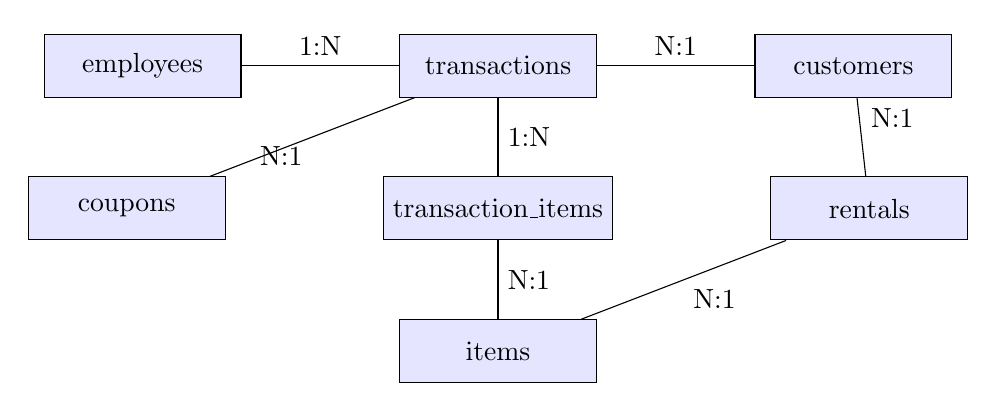
\begin{tikzpicture}[
    node distance=1cm,
    entity/.style={rectangle, draw, fill=blue!10, minimum width=2.5cm, minimum height=0.8cm},
]
    \node[entity] (emp) {employees};
    \node[entity, right=2cm of emp] (txn) {transactions};
    \node[entity, right=2cm of txn] (cust) {customers};
    \node[entity, below=of txn] (txnitem) {transaction\_items};
    \node[entity, below=of txnitem] (item) {items};
    \node[entity, left=2cm of txnitem] (coupon) {coupons};
    \node[entity, right=2cm of txnitem] (rental) {rentals};
    
    \draw[-] (emp) -- (txn) node[midway, above] {1:N};
    \draw[-] (txn) -- (cust) node[midway, above] {N:1};
    \draw[-] (txn) -- (txnitem) node[midway, right] {1:N};
    \draw[-] (txnitem) -- (item) node[midway, right] {N:1};
    \draw[-] (txn) -- (coupon) node[midway, below left] {N:1};
    \draw[-] (rental) -- (cust) node[midway, above right] {N:1};
    \draw[-] (rental) -- (item) node[midway, below right] {N:1};
\end{tikzpicture}
\caption{Entity Relationship Diagram}
\label{fig:erd}
\end{figure}

\end{document}
